



%\begin{figure}
%<<india-plot, echo = FALSE, fig = TRUE>>=
%
%a <- tapply(1:nrow(x), x$distH, function(i) x[i[order(x[i, "stunting"])],])
%a <- do.call("rbind", a)
%
%print(xyplot(p ~ stunting, groups = distH, data = a, type = "l",
%             col = rgb(.1, .1, .1, .1)))
%@
%\caption{India}
%\end{figure}


\setlength{\unitlength}{.9\textwidth}  % measure in textwidths

\begin{figure}
\begin{center}
  \begin{picture}(1,1)(.2, .0)
     \put(0,0){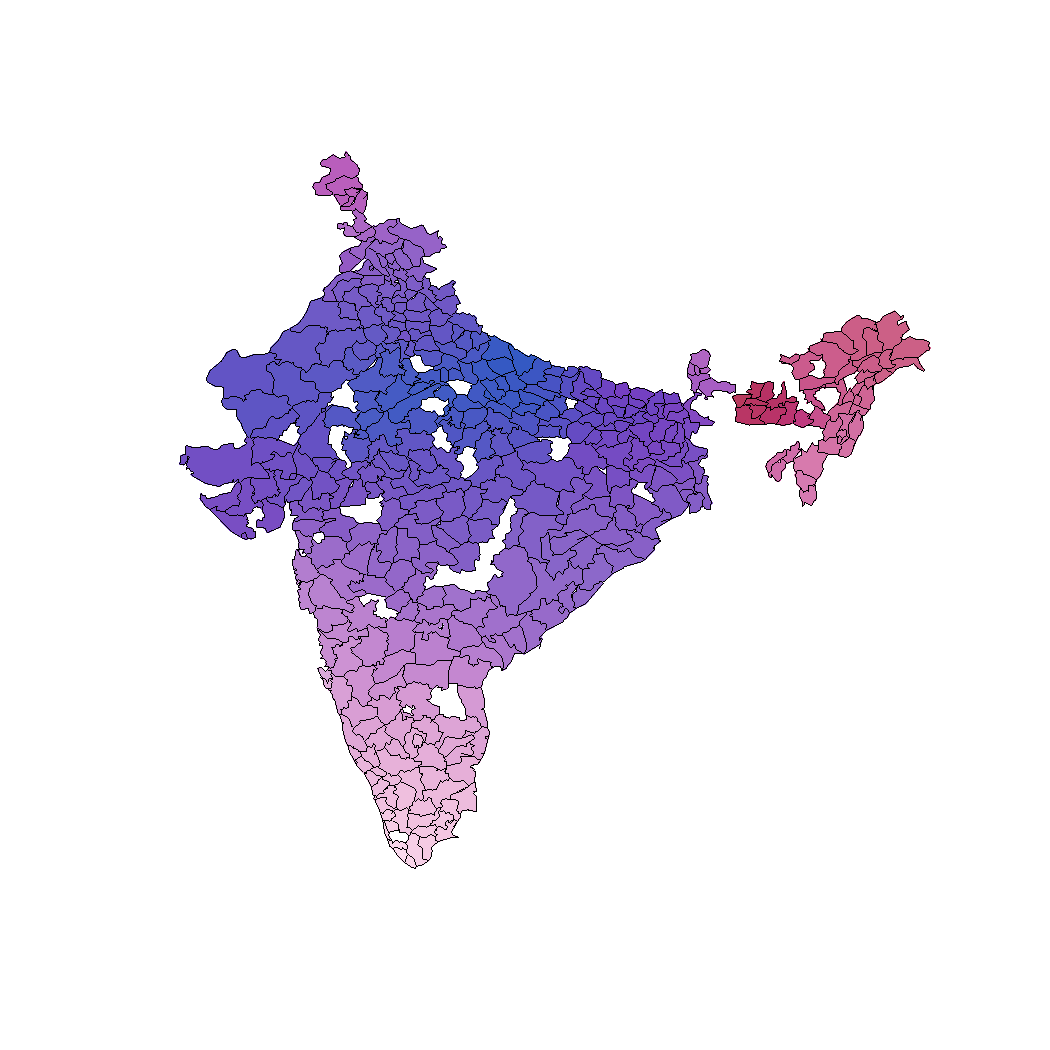
\includegraphics{figures/fig-india.pdf}}
     \put(.7,.2){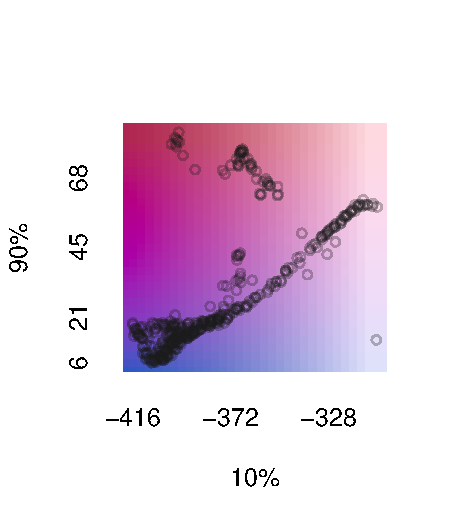
\includegraphics[width=.35\textwidth]{figures/fig-india-legend.pdf}}
  \end{picture}
\end{center}
\caption{Childhood Nutrition in India. Colour-coded map of the $10\%$ and $90\%$
         conditional quantiles of the $Z$ score. Each dot in the colour legend
         corresponds to one district with the respective colour in the map.
         Blue values in the northern part
         of India correspond to small lower and upper quantiles. Red values,
         especially in the eastern Meghalaya and Assam states, indicate small
         lower quantiles but at the same time large upper quantiles. In the southern part
         of India, the lower quantiles are largest with moderate upper quantiles.
         White parts indicate districts with no observations.
         \label{india_qplot}}
\end{figure}
